\documentclass[11pt]{paper}
\usepackage{palatino}
\usepackage{amsfonts,amsmath,amssymb}
% \usepackage{graphicx}

\usepackage{listings}
\usepackage{textcomp}
\usepackage{color}

\definecolor{dkgreen}{rgb}{0,0.6,0}
\definecolor{gray}{rgb}{0.5,0.5,0.5}
\definecolor{mauve}{rgb}{0.58,0,0.82}

\lstset{frame=tb,
  language=R,
  aboveskip=3mm,
  belowskip=3mm,
  showstringspaces=false,
  columns=flexible,
  basicstyle={\small\ttfamily},
  numbers=none,
  numberstyle=\tiny\color{gray},
  keywordstyle=\color{blue},
  commentstyle=\color{dkgreen},
  stringstyle=\color{mauve},
  breaklines=true,
  breakatwhitespace=true,
  tabsize=3
}



\ifx\pdftexversion\undefined
    \usepackage[dvips]{graphicx}
\else
    \usepackage[pdftex]{graphicx}
    \usepackage{epstopdf}
    \epstopdfsetup{suffix=}
\fi

\usepackage{subfig}

\begin{document}

%%%%%%%%%%%%%%%%%%%%%%%%%%%%%%%%%%%%%%%%
% Problem Set 7
%%%%%%%%%%%%%%%%%%%%%%%%%%%%%%%%%%%%%%%%

\pagestyle{empty}
{\noindent\bf Spring 2023 \hfill Firstname M.~Lastname}
\vskip 16pt
\centerline{\bf University of Central Florida}
\centerline{\bf College of Business}
\vskip 16pt
\centerline{\bf QMB 6911}
\centerline{\bf Capstone Project in Business Analytics}
\vskip 10pt
\centerline{\bf Solutions:  Problem Set \#6}
\vskip 32pt
\noindent

\section{Data Description}

This analysis follows the script \texttt{Tractor\_Reg\_Model.R} to produce a more accurate model for used tractor prices with the data from \texttt{TRACTOR7.csv} in the \texttt{Data} folder. 
The dataset includes the following variables.
\begin{table}[h!]
\begin{tabular}{l l l}

$saleprice_i$ & = & the price paid for tractor $i$ in dollars \\
% 
$horsepower_i$ & = & the horsepower of tractor $i$ \\
$age_i$ & = & the number of years since tractor $i$ was manufactured  \\
$enghours_i$ & = & the number of hours of use recorded for tractor $i$  \\
$diesel_i$ & = & an indicator of whether tractor $i$ runs on diesel fuel \\ %, $0$ otherwise \\
$fwd_i$ & = & an indicator of whether tractor $i$ has four-wheel drive \\ %, $0$ otherwise \\
$manual_i$ & = & an indicator of whether tractor $i$ has a manual transmission \\ %, $0$ otherwise \\
$johndeere_i$ & = & an indicator of whether tractor $i$ is manufactured by John Deere \\ %, $0$ otherwise \\
$cab_i$ & = & an indicator of whether tractor $i$ has an enclosed cab \\ %, $0$ otherwise \\
% 
$spring_i$ & = & an indicator of whether tractor $i$ was sold in April or May \\ %, $0$ otherwise \\
$summer_i$ & = & an indicator of whether tractor $i$ was sold between June and September \\ %, $0$ otherwise \\
$winter_i$ & = & an indicator of whether tractor $i$ was sold between December and March \\ %, $0$ otherwise \\

\end{tabular}
\end{table}
%

I will first estimate a model with our choices of functional form, and then consider exclusions of insignificant variables from the full model. 
This approach allows for inclusion of possibly irrelevant variables and avoids excluding any relevant variables. 


%%%%%%%%%%%%%%%%%%%%%%%%%%%%%%%%%%%%%%%%
% Choosing the Dependent Variable
%%%%%%%%%%%%%%%%%%%%%%%%%%%%%%%%%%%%%%%%


\pagebreak
\section{Choosing the Dependent Variable}

\subsection{Univariate Analysis}

Figure \ref{fig:hist_price} shows  a histogram of tractor prices.
The distribution is highly skewed to the right, 
with most tractors selling for about \$10,000 or less,
and very few tractors priced above \$50,000.



\begin{figure}[h!]
  \centering
  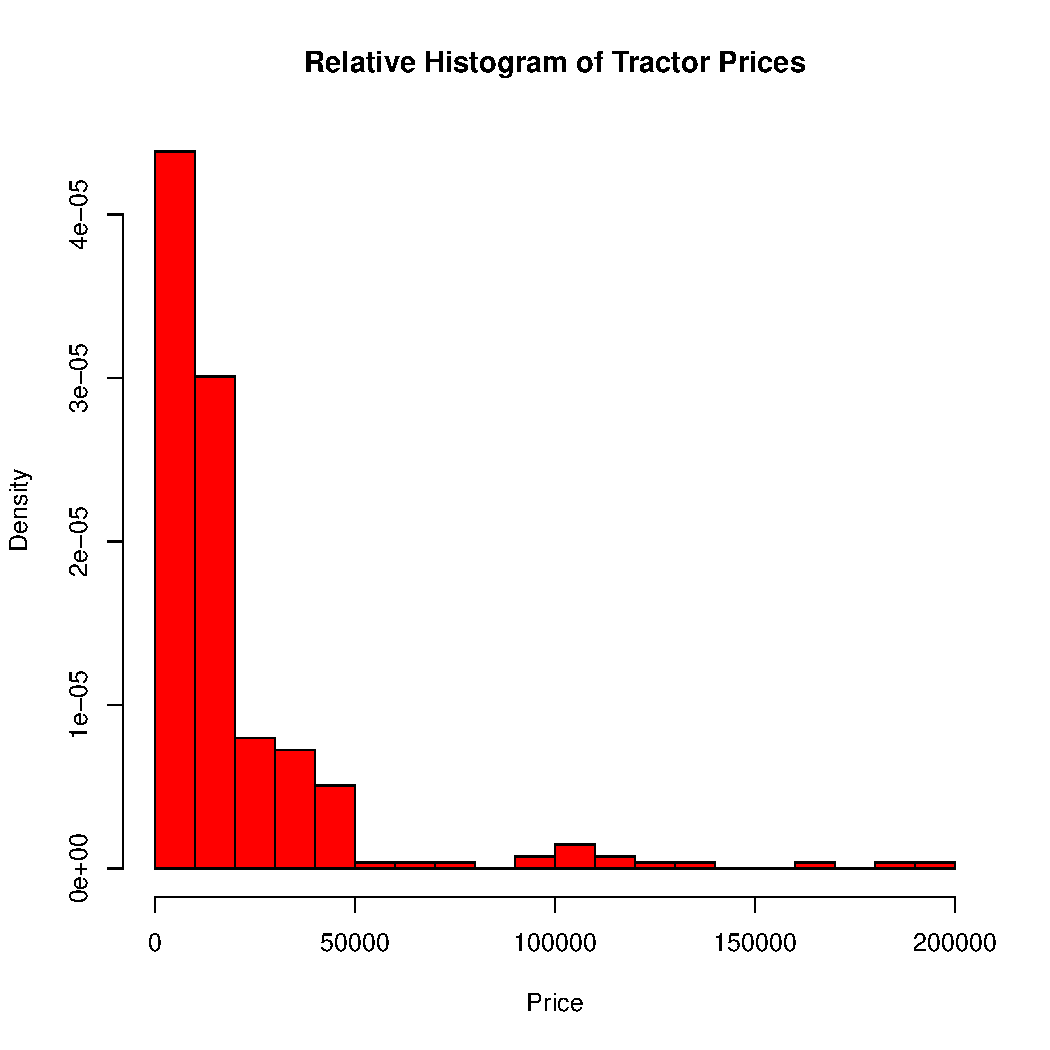
\includegraphics[scale = 0.5, keepaspectratio=true]{../Figures/hist_price}
  \caption{Histogram of Tractor Prices} \label{fig:hist_price}
\end{figure}



\pagebreak
As a comparison, Figure \ref{fig:hist_log_price} shows the histogram of the natural logarithm of
price.

\begin{figure}[h!]
  \centering
  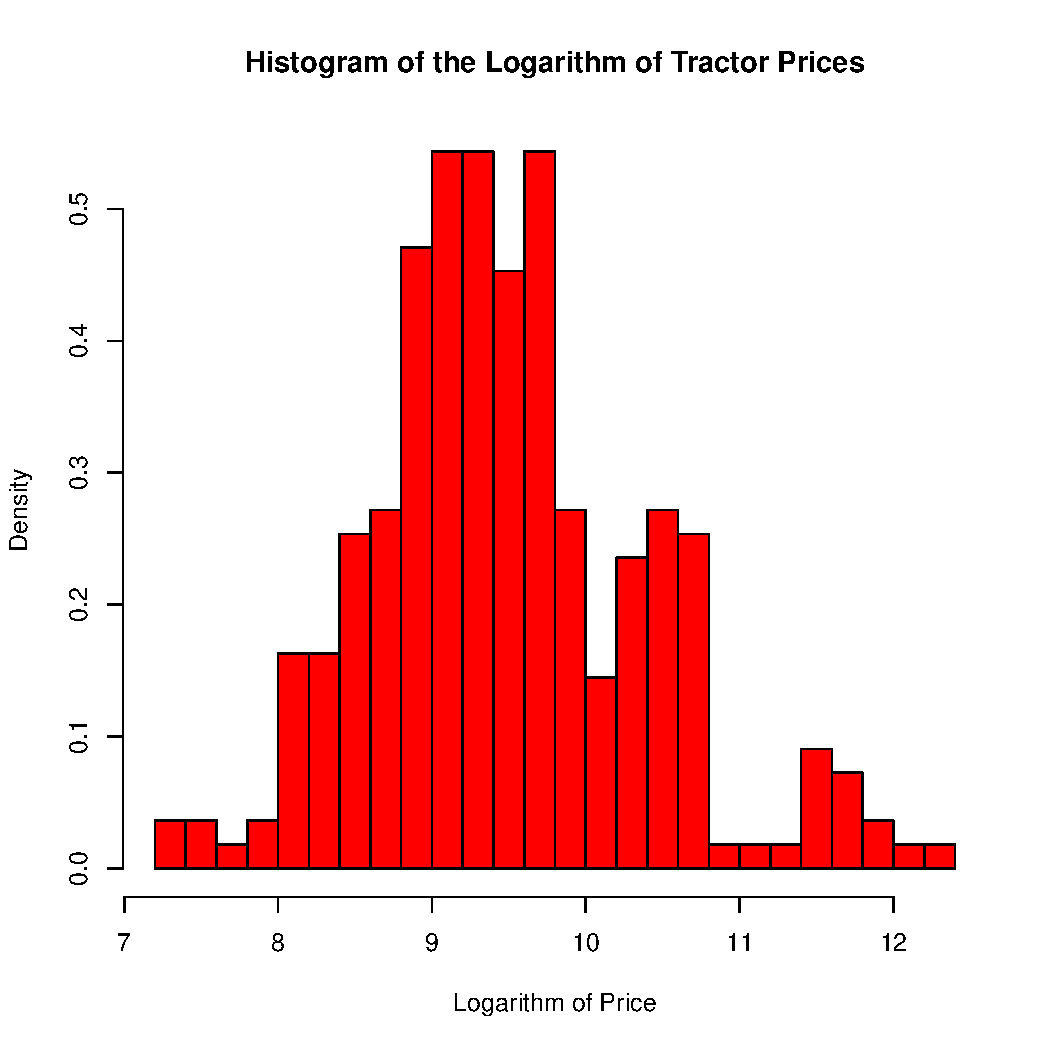
\includegraphics[scale = 0.5, keepaspectratio=true]{../Figures/hist_log_price}
  \caption{Histogram of the Logarithm of Tractor Prices} \label{fig:hist_log_price}
\end{figure}

This is much better behaved. The distribution looks almost normal. 
So far it looks as if the logarithm of the sale price
is the more promising variable.
Another approach to making this decision is
to build the model and judge the validity of the results.



%%%%%%%%%%%%%%%%%%%%%%%%%%%%%%%%%%%%%%%%
% Linear Regression Models
%%%%%%%%%%%%%%%%%%%%%%%%%%%%%%%%%%%%%%%%


\pagebreak
\subsection{Initial Regression Models of Tractor Prices}

\subsubsection{Predicting Price Levels}

First, I will build a model of the price of a used tractor, 
ignoring the above evidence that the distribution is highly skewed. 


\begin{table}
\begin{center}
\begin{tabular}{l c}
\hline
 & Model 1 \\
\hline
(Intercept) & $11670.41^{*}$   \\
            & $(4519.29)$      \\
horsepower  & $246.40^{***}$   \\
            & $(13.98)$        \\
age         & $-674.64^{***}$  \\
            & $(149.00)$       \\
enghours    & $-1.76^{***}$    \\
            & $(0.40)$         \\
diesel      & $2731.97$        \\
            & $(3996.05)$      \\
fwd         & $2570.57$        \\
            & $(2427.51)$      \\
manual      & $-3713.28$       \\
            & $(2586.96)$      \\
johndeere   & $12194.23^{***}$ \\
            & $(2979.91)$      \\
spring      & $-1721.01$       \\
            & $(2716.03)$      \\
summer      & $-5569.46^{*}$   \\
            & $(2654.94)$      \\
winter      & $-1541.99$       \\
            & $(2981.31)$      \\
\hline
R$^2$       & $0.65$           \\
Adj. R$^2$  & $0.63$           \\
Num. obs.   & $276$            \\
\hline
\multicolumn{2}{l}{\scriptsize{$^{***}p<0.001$; $^{**}p<0.01$; $^{*}p<0.05$}}
\end{tabular}
\caption{Dollar Value of Tractor Prices}
\label{tab:price_reg_1}
\end{center}
\end{table}


The results in Table \ref{tab:price_reg_1}
shows the effect of the variables on the dollar price of the
used tractors. 

From the coefficients in the table, 
it appears that a John Deere tractor sells for 
\$12,200 more than an equivalent tractor of another brand. 
This prediction applies equally for tractors all across the spectrum, from the 
To put a finer point on it, 
a 16 horsepower lawn tractor that would otherwise sell for \$2,000 is expected to command \$14,200 if it is a John Deere.
Clearly, this is an unreasonable expectation and
a quick search on your browser will confirm that the John Deere premium is more modest. 


\pagebreak
\subsubsection{Predicting Logarithm of Prices}

Next, I will build a model of the logarithm of the price 
of a used tractor, 
which is consistent with the univariate analysis we conducted earlier. 


\begin{table}
\begin{center}
\begin{tabular}{l c}
\hline
 & Model 1 \\
\hline
(Intercept) & $8.76953^{***}$  \\
            & $(0.13528)$      \\
horsepower  & $0.00654^{***}$  \\
            & $(0.00042)$      \\
age         & $-0.02754^{***}$ \\
            & $(0.00446)$      \\
enghours    & $-0.00002$       \\
            & $(0.00001)$      \\
diesel      & $0.49917^{***}$  \\
            & $(0.11962)$      \\
fwd         & $0.35672^{***}$  \\
            & $(0.07266)$      \\
manual      & $-0.12167$       \\
            & $(0.07744)$      \\
johndeere   & $0.17253$        \\
            & $(0.08920)$      \\
spring      & $-0.03210$       \\
            & $(0.08130)$      \\
summer      & $-0.11876$       \\
            & $(0.07947)$      \\
winter      & $0.04009$        \\
            & $(0.08924)$      \\
\hline
R$^2$       & $0.69709$        \\
Adj. R$^2$  & $0.68566$        \\
Num. obs.   & $276$            \\
\hline
\multicolumn{2}{l}{\scriptsize{$^{***}p<0.001$; $^{**}p<0.01$; $^{*}p<0.05$}}
\end{tabular}
\caption{Logarithm of Tractor Prices}
\label{tab:log_price_reg_2}
\end{center}
\end{table}


The results in Table \ref{tab:log_price_reg_2}
shows the effect of the variables on the logarithm of the dollar price of the used tractors. 
This specification calculates coefficients that 
approximately represent percentage changes in 
tractor prices. 

From the coefficients in the table, 
it appears that a John Deere tractor sells for 
17\% more than an equivalent tractor of another brand. 
That is, a tractor worth \$1,700 would sell
for \$2,000 if it is a John Deere, 
which is clearly more reasonable. 
This more sensible interpretation supports 
the strategy of modeling the 
logarithm of the tractor price. 


%%%%%%%%%%%%%%%%%%%%%%%%%%%%%%%%%%%%%%%%
\clearpage
\section{Model Specification}
%%%%%%%%%%%%%%%%%%%%%%%%%%%%%%%%%%%%%%%%

\subsection{Initial Variable Reduction}

Next, I can refine the model by removing some explanatory variables that do not have string predictive value.
The first candidates are those with coefficients that are not statistically significant. 
The results in Table \ref{tab:reg_reduction}


\begin{table}
\begin{center}
\begin{tabular}{l c c c}
\hline
 & Model 1 & Model 2 & Model 3 \\
\hline
(Intercept) & $8.7695^{***}$  & $8.7559^{***}$  & $8.7787^{***}$  \\
            & $(0.1353)$      & $(0.1284)$      & $(0.1279)$      \\
horsepower  & $0.0065^{***}$  & $0.0066^{***}$  & $0.0065^{***}$  \\
            & $(0.0004)$      & $(0.0004)$      & $(0.0004)$      \\
age         & $-0.0275^{***}$ & $-0.0278^{***}$ & $-0.0297^{***}$ \\
            & $(0.0045)$      & $(0.0044)$      & $(0.0043)$      \\
enghours    & $-0.0000$       & $-0.0000$       & $-0.0000$       \\
            & $(0.0000)$      & $(0.0000)$      & $(0.0000)$      \\
diesel      & $0.4992^{***}$  & $0.4884^{***}$  & $0.4246^{***}$  \\
            & $(0.1196)$      & $(0.1192)$      & $(0.1118)$      \\
fwd         & $0.3567^{***}$  & $0.3492^{***}$  & $0.3416^{***}$  \\
            & $(0.0727)$      & $(0.0721)$      & $(0.0721)$      \\
manual      & $-0.1217$       & $-0.1169$       &                 \\
            & $(0.0774)$      & $(0.0773)$      &                 \\
johndeere   & $0.1725$        & $0.1858^{*}$    & $0.1707$        \\
            & $(0.0892)$      & $(0.0888)$      & $(0.0885)$      \\
spring      & $-0.0321$       &                 &                 \\
            & $(0.0813)$      &                 &                 \\
summer      & $-0.1188$       &                 &                 \\
            & $(0.0795)$      &                 &                 \\
winter      & $0.0401$        &                 &                 \\
            & $(0.0892)$      &                 &                 \\
\hline
R$^2$       & $0.6971$        & $0.6934$        & $0.6907$        \\
Adj. R$^2$  & $0.6857$        & $0.6853$        & $0.6838$        \\
Num. obs.   & $276$           & $276$           & $276$           \\
\hline
\multicolumn{4}{l}{\scriptsize{$^{***}p<0.001$; $^{**}p<0.01$; $^{*}p<0.05$}}
\end{tabular}
\caption{Models for the Log. of Tractor Prices}
\label{tab:reg_reduction}
\end{center}
\end{table}


The first column of Table \ref{tab:reg_reduction}
shows the results from the original model of
the logarithm of tractor prices in Table \ref{tab:log_price_reg_2}. 
The coefficients for seasonal indicators, 
engine hours and manual transmission are not significant.
The John Deere indicator is not significant
but since it is a key empirical question, 
I include it, regardless. 
The second column shows the model without the seasonal indicators. 
We see an improvement in significance of
some variables with minimal loss of predictive ability. 
In the last column, I remove the indicator for manual transmission, with a similar effect on the quality of the model. 
Before making any further changes, 
I will improve the specification of the model
by considering nonlinear specifications. 

\clearpage
\subsection{Quadratic Specification for Horsepower}

Now suppose that 
a used tractor dealer reports that overpowered used tractors are hard to sell, since they consume more fuel. 
This implies that tractor prices often increase with horsepower, up to a point, but beyond that they decrease. 
To incorporate this advice, I created and included a variable for squared horsepower. 

If we expect a decreasing relationship for high values of horsepower, 
this would be characterized by 
a positive coefficient on the horsepower variable and
a negative coefficient on the squared horsepower variable. 

The results of this regression specification are shown in 
Table \ref{tab:reg_sq_horse}. 
% 

\begin{table}
\begin{center}
\begin{tabular}{l c c c}
\hline
 & Model 1 & Model 2 & Model 3 \\
\hline
(Intercept)         & $8.60684^{***}$  & $8.72555^{***}$  & $8.72792^{***}$  \\
                    & $(0.11233)$      & $(0.11156)$      & $(0.10602)$      \\
horsepower          & $0.01504^{***}$  & $0.01115^{***}$  & $0.01112^{***}$  \\
                    & $(0.00097)$      & $(0.00107)$      & $(0.00107)$      \\
squared\_horsepower & $-0.00002^{***}$ & $-0.00001^{***}$ & $-0.00001^{***}$ \\
                    & $(0.00000)$      & $(0.00000)$      & $(0.00000)$      \\
age                 & $-0.03429^{***}$ & $-0.03206^{***}$ & $-0.03233^{***}$ \\
                    & $(0.00374)$      & $(0.00359)$      & $(0.00358)$      \\
enghours            & $-0.00004^{***}$ & $-0.00004^{***}$ & $-0.00004^{***}$ \\
                    & $(0.00001)$      & $(0.00001)$      & $(0.00001)$      \\
diesel              & $0.20070^{*}$    & $0.21453^{*}$    & $0.20350^{*}$    \\
                    & $(0.09975)$      & $(0.09854)$      & $(0.09805)$      \\
fwd                 & $0.31288^{***}$  & $0.27526^{***}$  & $0.26539^{***}$  \\
                    & $(0.06259)$      & $(0.05876)$      & $(0.05820)$      \\
johndeere           & $0.23842^{**}$   & $0.30972^{***}$  & $0.31872^{***}$  \\
                    & $(0.07705)$      & $(0.07236)$      & $(0.07186)$      \\
manual              &                  & $-0.15308^{*}$   & $-0.15015^{*}$   \\
                    &                  & $(0.06209)$      & $(0.06189)$      \\
cab                 &                  & $0.47786^{***}$  & $0.48345^{***}$  \\
                    &                  & $(0.07031)$      & $(0.07003)$      \\
spring              &                  & $-0.04892$       &                  \\
                    &                  & $(0.06506)$      &                  \\
summer              &                  & $-0.05729$       &                  \\
                    &                  & $(0.06379)$      &                  \\
winter              &                  & $0.04596$        &                  \\
                    &                  & $(0.07141)$      &                  \\
\hline
R$^2$               & $0.76838$        & $0.80761$        & $0.80591$        \\
Adj. R$^2$          & $0.76233$        & $0.79884$        & $0.79935$        \\
Num. obs.           & $276$            & $276$            & $276$            \\
\hline
\multicolumn{4}{l}{\scriptsize{$^{***}p<0.001$; $^{**}p<0.01$; $^{*}p<0.05$}}
\end{tabular}
\caption{Quadratic Models for Tractor Prices}
\label{tab:reg_sq_horse}
\end{center}
\end{table}

% 
The squared horsepower variable has a coefficient of $-2.081e-05$, which is nearly ten times as large as the standard error of $2.199e-06$, which is very strong evidence against the null hypothesis of a positive or zero coefficient. 
I conclude that the log of the sale price does decline for large values of horsepower. 


With the squared horsepower variable, the $\bar{R}^2$ has increased substantially to $0.764$, indicating that it is a much stronger model. 
The $F$-statistic is even larger than before, indicating that it is still a better candidate than the simple average log sale price. 
The new squared horsepower variable is statistically significant and the theory behind it is sound, since above a certain point, added horsepower may not improve performance but will cost more to operate. 
This new model is much improved over the previous models with a linear specification for horsepower.

This improved model affords an opportunity
to reconsider other variables in the previous models.
Models 2 and 3 both include an indicator that the
tractor has an enclosed cab, 
which is also statistically significant. 
The seasonal indicators in Model 2 are not statistically significant under this specification neither. 

\clearpage
\subsection{Seasonality with the Quadratic Specification for Horsepower}


The seasonal indicators in Model 2 
of Table \ref{tab:reg_sq_horse}
are not statistically significant individually.
It is possible, however, that jointly, they 
offer an improvement in prediction. 
This can be tested with an $F$-test
to test the joint hypothesis that the time of year has no effect on the sale of tractors. 
%
The null hypothesis is the joint hypothesis that all coefficients on spring, summer and winter are equal to zero. 
The alternative hypothesis is that one of these coefficients is nonzero. 
% 

From the script \texttt{Tractor\_Reg\_Models.R}, the Residual Sum of Squares from the unconstrained model (the model which includes the seasonal indicators) is $41.78944$. 
The constrained model is the one that excludes seasonal indicators and it has a Residual Sum of Squares of $42.15882$.

The $F$-statistic has a value of 

$$ 
\frac{(RSS_M - RSS)/M}{RSS/(N - K - 1)} = \frac{(42.15882 - 41.78944)/3}{RSS/263} = 0.7748937. 
$$

since $N = 276$ observations, $K = 12$ variables and $M = 3$ restrictions, one for each seasonal indicator excluded. 
This is a low value compared to the critical value of $2.60$ for the $F$-statistic with $3$ degrees of freedom in the numerator and $263 (> 120)$ degrees of freedom in the denominator. 
There is no evidence to reject the null that all seasonal indicators have coefficients of zero and conclude that the seasonal indicators should be left out of the model. 
%
The results of the test above indicate that tractor prices do not follow a seasonal pattern. 


\clearpage
\subsection{Interaction Terms}

\subsubsection{Durability of Engine Types}

Finally, I consider another modification to your model. 
Diesel engines tend to be more durable than gasoline engines. 
This raises the question of whether an additional hour of use affects the value of a diesel tractor differently than for a gasoline tractor. 
This is tested in Model 1 of Table \ref{tab:reg_interactions}. 

	This hypothesis is a test of the \emph{interaction} of the diesel indicator and the slope on engine hours. 
      Given the above result, this test should be conducted with the model that excludes the seasonal indicators. 
The coefficient on \texttt{enghours:diesel} is $4.116e-06$ with a standard error of $2.736e-05$, resulting in a $t$-statistic of $0.150$. 
Since this is a very low value, we cannot reject the null hypothesis that an additional hour of use affects the value of a diesel tractor the same as that for a gasoline tractor. 
Note that this conclusion does not change if you test a one-sided hypothesis.  

Furthermore, the $\bar{R}^2$ statistic decreases with the inclusion of this variable. 
The $F$-statistic is high and statistically significant, indicating that this model is better than the simple average but so is the model without this new variable. 
Finally, the estimates of the other coefficients change very little when this variable is omitted. 
The theory may be sound but there is nothing else to support the inclusion of this new variable. 

% \clearpage
\pagebreak
\subsubsection{Differences in Depreciation by Brand}

The remaining columns of Table \ref{tab:reg_interactions}
show the results of tests for interactions
between the John Deere indicator variable
on the effects of age, engine hours and horsepower. 
There seems to be no evidence for relationships that differ by
brand name. 
In this table, we have investigated several 
individual types of differences by brand. 


\begin{table}
\begin{center}
\begin{tabular}{l c c c c}
\hline
 & Model 1 & Model 2 & Model 3 & Model 4 \\
\hline
(Intercept)          & $8.89189^{***}$  & $8.88028^{***}$  & $8.87926^{***}$  & $8.89127^{***}$  \\
                     & $(0.12827)$      & $(0.11042)$      & $(0.11163)$      & $(0.11165)$      \\
horsepower           & $0.00488^{***}$  & $0.00490^{***}$  & $0.00489^{***}$  & $0.00476^{***}$  \\
                     & $(0.00039)$      & $(0.00039)$      & $(0.00039)$      & $(0.00043)$      \\
age                  & $-0.02986^{***}$ & $-0.02994^{***}$ & $-0.02990^{***}$ & $-0.02969^{***}$ \\
                     & $(0.00381)$      & $(0.00381)$      & $(0.00400)$      & $(0.00381)$      \\
enghours             & $-0.00004$       & $-0.00004^{***}$ & $-0.00004^{***}$ & $-0.00004^{***}$ \\
                     & $(0.00003)$      & $(0.00001)$      & $(0.00001)$      & $(0.00001)$      \\
diesel               & $0.28447^{*}$    & $0.30271^{**}$   & $0.29874^{**}$   & $0.29293^{**}$   \\
                     & $(0.12619)$      & $(0.10378)$      & $(0.10389)$      & $(0.10387)$      \\
fwd                  & $0.25952^{***}$  & $0.25727^{***}$  & $0.25879^{***}$  & $0.26050^{***}$  \\
                     & $(0.06238)$      & $(0.06230)$      & $(0.06229)$      & $(0.06226)$      \\
manual               & $-0.16119^{*}$   & $-0.15793^{*}$   & $-0.16018^{*}$   & $-0.16217^{*}$   \\
                     & $(0.06631)$      & $(0.06632)$      & $(0.06692)$      & $(0.06619)$      \\
johndeere            & $0.31091^{***}$  & $0.25824^{*}$    & $0.30345^{*}$    & $0.24957^{*}$    \\
                     & $(0.07868)$      & $(0.11399)$      & $(0.15228)$      & $(0.10998)$      \\
cab                  & $0.67506^{***}$  & $0.67717^{***}$  & $0.67571^{***}$  & $0.67665^{***}$  \\
                     & $(0.06732)$      & $(0.06728)$      & $(0.06734)$      & $(0.06722)$      \\
enghours:diesel      & $0.00001$        &                  &                  &                  \\
                     & $(0.00003)$      &                  &                  &                  \\
enghours:johndeere   &                  & $0.00001$        &                  &                  \\
                     &                  & $(0.00002)$      &                  &                  \\
age:johndeere        &                  &                  & $0.00023$        &                  \\
                     &                  &                  & $(0.00742)$      &                  \\
horsepower:johndeere &                  &                  &                  & $0.00057$        \\
                     &                  &                  &                  & $(0.00077)$      \\
\hline
R$^2$                & $0.77769$        & $0.77795$        & $0.77766$        & $0.77811$        \\
Adj. R$^2$           & $0.77017$        & $0.77043$        & $0.77014$        & $0.77060$        \\
Num. obs.            & $276$            & $276$            & $276$            & $276$            \\
\hline
\multicolumn{5}{l}{\scriptsize{$^{***}p<0.001$; $^{**}p<0.01$; $^{*}p<0.05$}}
\end{tabular}
\caption{Regression Models for Tractor Prices}
\label{tab:reg_interactions}
\end{center}
\end{table}


To test for many possible differences in 
models by brand of tractor, 
Table \ref{tab:reg_johndeere}
shows the estimates for two separate models
by brand of tractor.
%
Model 1 shows the estimates for 
the full sample,
Model 2 shows the estimates from the full model for 
John Deere tractors
and Model 4 
represents all other brands. 
% 
Models 3 and 5 show the estimates from a reduced version of each model, 
in which all coefficients are statistically significant. 
% 
The coefficients appear similar across the two subsamples.
Notable differences include the statistical significance for 
the indicators for four-wheel drive, 
manual transmission and an enclosed cab. 
These features seem to change the value of 
other tractors, but perhaps these coefficients are not measured 
accurately for the small sample of 39 
John Deere tractors. 


\begin{table}
\begin{center}
\begin{tabular}{l c c c c c}
\hline
 & Model 1 & Model 2 & Model 3 & Model 4 & Model 5 \\
\hline
(Intercept)         & $8.72792^{***}$  & $8.86706^{***}$  & $9.03796^{***}$  & $8.77320^{***}$  & $8.90792^{***}$  \\
                    & $(0.10602)$      & $(0.22409)$      & $(0.16430)$      & $(0.12450)$      & $(0.08769)$      \\
horsepower          & $0.01112^{***}$  & $0.01502^{***}$  & $0.01580^{***}$  & $0.01032^{***}$  & $0.01057^{***}$  \\
                    & $(0.00107)$      & $(0.00250)$      & $(0.00223)$      & $(0.00119)$      & $(0.00119)$      \\
squared\_horsepower & $-0.00001^{***}$ & $-0.00002^{***}$ & $-0.00002^{***}$ & $-0.00001^{***}$ & $-0.00001^{***}$ \\
                    & $(0.00000)$      & $(0.00000)$      & $(0.00000)$      & $(0.00000)$      & $(0.00000)$      \\
age                 & $-0.03233^{***}$ & $-0.03038^{**}$  & $-0.03295^{***}$ & $-0.03164^{***}$ & $-0.03283^{***}$ \\
                    & $(0.00358)$      & $(0.00914)$      & $(0.00738)$      & $(0.00399)$      & $(0.00392)$      \\
enghours            & $-0.00004^{***}$ & $-0.00006^{*}$   & $-0.00006^{**}$  & $-0.00004^{***}$ & $-0.00004^{***}$ \\
                    & $(0.00001)$      & $(0.00002)$      & $(0.00002)$      & $(0.00001)$      & $(0.00001)$      \\
diesel              & $0.20350^{*}$    & $0.08485$        &                  & $0.18218$        &                  \\
                    & $(0.09805)$      & $(0.18242)$      &                  & $(0.11984)$      &                  \\
fwd                 & $0.26539^{***}$  & $0.12882$        &                  & $0.29072^{***}$  & $0.30003^{***}$  \\
                    & $(0.05820)$      & $(0.15529)$      &                  & $(0.06308)$      & $(0.06296)$      \\
manual              & $-0.15015^{*}$   & $0.06749$        &                  & $-0.17919^{**}$  & $-0.14668^{*}$   \\
                    & $(0.06189)$      & $(0.17288)$      &                  & $(0.06743)$      & $(0.06413)$      \\
johndeere           & $0.31872^{***}$  &                  &                  &                  &                  \\
                    & $(0.07186)$      &                  &                  &                  &                  \\
cab                 & $0.48345^{***}$  & $0.32344$        & $0.38517^{*}$    & $0.51732^{***}$  & $0.52756^{***}$  \\
                    & $(0.07003)$      & $(0.17555)$      & $(0.16365)$      & $(0.07696)$      & $(0.07688)$      \\
\hline
R$^2$               & $0.80591$        & $0.91993$        & $0.91606$        & $0.77992$        & $0.77769$        \\
Adj. R$^2$          & $0.79935$        & $0.89858$        & $0.90334$        & $0.77220$        & $0.77090$        \\
Num. obs.           & $276$            & $39$             & $39$             & $237$            & $237$            \\
\hline
\multicolumn{6}{l}{\scriptsize{$^{***}p<0.001$; $^{**}p<0.01$; $^{*}p<0.05$}}
\end{tabular}
\caption{Separate Models by Brand}
\label{tab:reg_johndeere}
\end{center}
\end{table}


We can also test for all of the differences at the same time
by using an $F$-test. 
In this case, the full, unrestricted model has $K = 2\times9 = 18$ parameters, one for each variable in two models. 
The test that all of the coefficients are the same has $M = 9 - 1 = 8$
restrictions. 
The one restriction fewer accounts for the John Deere indicator
in the full model, 
which allows for two separate intercepts. 
% 
The $F$-statistic has a value of 

$$ 
\frac{(RSS_M - RSS)/M}{RSS/(N - K - 1)} = \frac{(42.15882 - 41.1432)/3}{41.1432/263} = 0.7929991. 
$$

This is also a very low value for the $F$-statistic. 
There is no evidence to reject the null that all 
coefficients are equal across both samples 
and conclude that the John Deere indicator
should be the only brand difference left in the model. 

%%%%%%%%%%%%%%%%%%%%%%%%%%%%%%%%%%%%%%%%
\end{document}
%%%%%%%%%%%%%%%%%%%%%%%%%%%%%%%%%%%%%%%%
